\documentclass[11pt]{article}
\usepackage[margin=0.75in]{geometry}
\usepackage{amsmath,amssymb}
\usepackage{xcolor}
\usepackage{tikz}
\usepackage[most]{tcolorbox}
\usepackage{enumitem}
\usepackage{titlesec}
\usepackage{fancyhdr}

\definecolor{ink}{HTML}{1F3A5F}
\definecolor{key}{HTML}{8A1C1C}
\definecolor{soft}{HTML}{EEF3F8}
\definecolor{warm}{HTML}{FBF3E6}

\setlength{\parindent}{0pt}
\setlength{\parskip}{4pt}
\setlist{itemsep=1pt,topsep=2pt}
\titleformat{\section}{\large\bfseries\color{ink}}{\thesection.}{0.5em}{}
\titleformat{\subsection}{\normalsize\bfseries\color{ink}}{}{0em}{}
\titlespacing*{\section}{0pt}{10pt}{4pt}
\titlespacing*{\subsection}{0pt}{6pt}{2pt}

\newcommand{\E}{\mathrm{E}}

\newtcolorbox{bigidea}{colback=soft,colframe=ink,boxrule=0.6pt,arc=2pt,left=5pt,right=5pt,top=3pt,bottom=3pt,
  title={\bfseries\small Big idea},fonttitle=\small}
\newtcolorbox{trap}{colback=warm,colframe=key,boxrule=0.6pt,arc=2pt,left=5pt,right=5pt,top=3pt,bottom=3pt,
  title={\bfseries\small Traps / what graders look for},fonttitle=\small}
\newtcolorbox{answer}{colback=white,colframe=ink,boxrule=0.6pt,arc=2pt,left=6pt,right=6pt,top=4pt,bottom=4pt,
  title={\bfseries\small Model answer},fonttitle=\small,breakable}

\pagestyle{fancy}
\fancyhf{}
\renewcommand{\headrulewidth}{0pt}
\fancyfoot[C]{\small\thepage}

% Shared TikZ figures for the ECON 5040 midterm study guide and sample midterm.
% Each \fig... macro draws one self-contained tikzpicture.

% 1. Intertemporal budget line: R is minus the slope
\newcommand{\figIntertemporal}{%
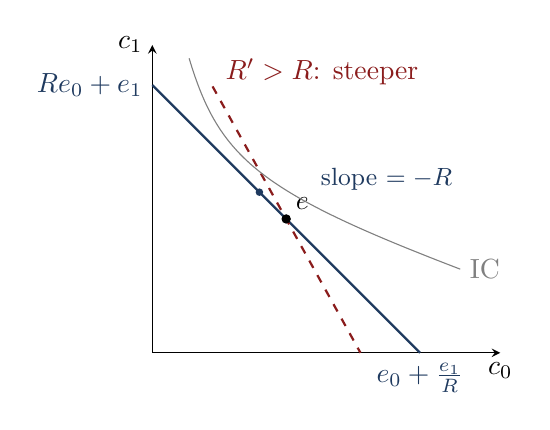
\begin{tikzpicture}[scale=0.85,>=stealth]
  \draw[->] (0,0) -- (5.2,0) node[below] {$c_0$};
  \draw[->] (0,0) -- (0,4.6) node[left] {$c_1$};
  % endowment e = (2,2); budget with R = 1 (slope -1) and R' > R (slope -1.8)
  \draw[thick,ink] (0,4) -- (4,0) node[below] {$e_0+\tfrac{e_1}{R}$};
  \node[left,ink] at (0,4) {$Re_0+e_1$};
  \draw[thick,key,dashed] (0.9,3.98) -- (3.11,0);
  \node[key,right] at (0.95,4.2) {$R'>R$: steeper};
  \fill (2,2) circle (2pt) node[above right] {$e$};
  % indifference curve tangent to the original line at (1.6,2.4)
  \draw[gray] (0.55,4.4) .. controls (1.0,2.9) and (1.6,2.4) .. (4.6,1.25);
  \fill[ink] (1.6,2.4) circle (1.6pt);
  \node[gray,right] at (4.6,1.25) {IC};
  \node[ink] at (3.5,2.6) {\small slope $=-R$};
\end{tikzpicture}}

% 2. Concave utility, expected utility, certainty equivalent
\newcommand{\figCE}{%
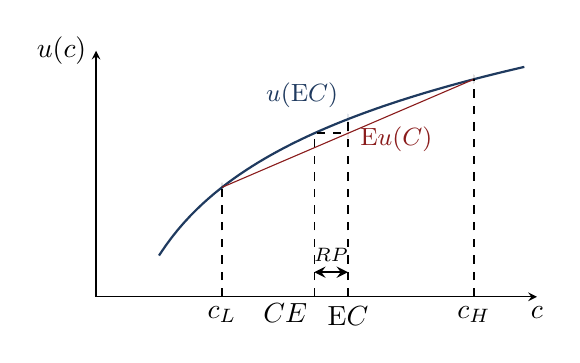
\begin{tikzpicture}[xscale=0.032,yscale=1.25,>=stealth]
  \draw[->] (0,2.8) -- (175,2.8) node[below] {$c$};
  \draw[->] (0,2.8) -- (0,5.3) node[left] {$u(c)$};
  \draw[thick,ink,domain=25:170,samples=60] plot (\x,{ln(\x)});
  \draw[key] (50,{ln(50)}) -- (150,{ln(150)});
  \fill (50,{ln(50)}) circle (1.4pt); \fill (150,{ln(150)}) circle (1.4pt);
  % E[C]=100, E[u]=0.5(ln50+ln150)=4.4637, CE=86.6, u(100)=4.6052
  \fill[key] (100,4.4637) circle (1.6pt);
  \fill[ink] (100,4.6052) circle (1.6pt);
  \draw[dashed] (100,2.8) node[below] {$\E C$} -- (100,4.6052);
  \draw[dashed] (86.6,2.8) node[below left=-1pt] {$CE$} -- (86.6,4.4637) -- (100,4.4637);
  \draw[dashed] (50,2.8) node[below] {$c_L$} -- (50,{ln(50)});
  \draw[dashed] (150,2.8) node[below] {$c_H$} -- (150,{ln(150)});
  \node[ink,above left] at (100,4.62) {\small $u(\E C)$};
  \node[key,right] at (101,4.40) {\small $\E u(C)$};
  \draw[<->,thick] (86.6,3.05) -- node[above] {\scriptsize $RP$} (100,3.05);
\end{tikzpicture}}

% 3. Two-state Markov chain
\newcommand{\figMarkov}{%
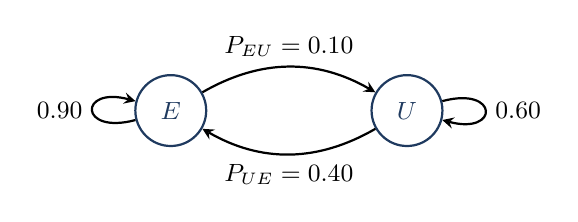
\begin{tikzpicture}[>=stealth,node distance=3cm,every node/.style={font=\small}]
  \node[circle,draw,thick,ink,minimum size=9mm] (E) {$E$};
  \node[circle,draw,thick,ink,minimum size=9mm,right of=E] (U) {$U$};
  \draw[->,thick] (E) to[bend left] node[above] {$P_{EU}=0.10$} (U);
  \draw[->,thick] (U) to[bend left] node[below] {$P_{UE}=0.40$} (E);
  \draw[->,thick] (E) to[loop left] node[left] {$0.90$} (E);
  \draw[->,thick] (U) to[loop right] node[right] {$0.60$} (U);
\end{tikzpicture}}

% 4. Bellman decomposition / timing
\newcommand{\figBellman}{%
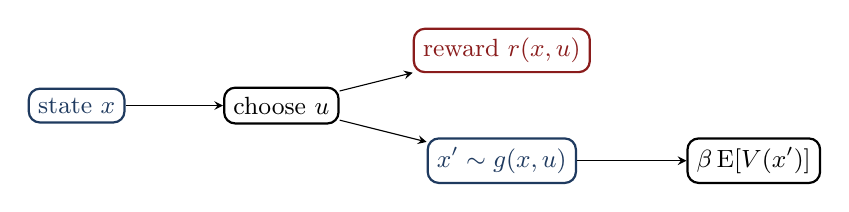
\begin{tikzpicture}[>=stealth,every node/.style={font=\small}]
  \node[draw,rounded corners,ink,thick] (x) at (0,0) {state $x$};
  \node[draw,rounded corners,thick] (u) at (2.6,0) {choose $u$};
  \node[draw,rounded corners,key,thick] (r) at (5.4,0.7) {reward $r(x,u)$};
  \node[draw,rounded corners,ink,thick] (xp) at (5.4,-0.7) {$x'\sim g(x,u)$};
  \node[draw,rounded corners,thick] (v) at (8.6,-0.7) {$\beta\,\E[V(x')]$};
  \draw[->] (x) -- (u); \draw[->] (u) -- (r); \draw[->] (u) -- (xp); \draw[->] (xp) -- (v);
\end{tikzpicture}}

% 5. Solow: sf(k) vs delta k, with a rise in s
\newcommand{\figSolow}{%
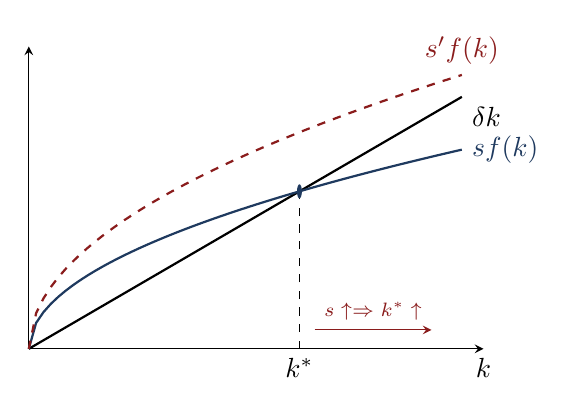
\begin{tikzpicture}[xscale=0.55,yscale=1.6,>=stealth]
  \draw[->] (0,0) -- (10.5,0) node[below] {$k$};
  \draw[->] (0,0) -- (0,2.4);
  \draw[thick] (0,0) -- (10,2) node[below right] {$\delta k$};
  \draw[thick,ink,domain=0:10,samples=60] plot (\x,{0.4*sqrt(\x)*1.25}) node[right] {$sf(k)$};
  \draw[thick,key,dashed,domain=0:10,samples=60] plot (\x,{0.55*sqrt(\x)*1.25}) node[above] {$s'f(k)$};
  % k* where 0.5 sqrt k = 0.2 k -> k = 6.25 ; k*' where 0.6875 sqrt k = 0.2k -> k = 11.8 (off-axis) so use 0.55*1.25=0.6875
  \draw[dashed] (6.25,0) node[below] {$k^*$} -- (6.25,1.25);
  \fill[ink] (6.25,1.25) circle (1.6pt);
  \draw[->,key] (6.6,0.15) -- (9.3,0.15) node[midway,above] {\scriptsize $s\uparrow\Rightarrow k^*\uparrow$};
  
\end{tikzpicture}}

% 6. Level effect vs growth effect
\newcommand{\figLevelGrowth}{%
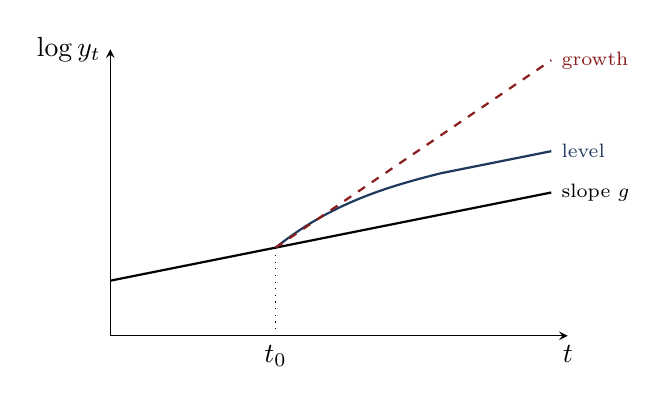
\begin{tikzpicture}[xscale=0.7,yscale=0.7,>=stealth]
  \draw[->] (0,0) -- (8.3,0) node[below] {$t$};
  \draw[->] (0,0) -- (0,5.2) node[left] {$\log y_t$};
  \draw[thick] (0,1) -- (8,2.6) node[right] {\scriptsize slope $g$};
  \draw[thick,ink] (3,1.6) .. controls (4,2.4) and (5,2.7) .. (6,2.95) -- (8,3.35) node[right] {\scriptsize level};
  \draw[thick,key,dashed] (3,1.6) -- (8,5.0) node[right] {\scriptsize growth};
  \draw[dotted] (3,0) node[below] {$t_0$} -- (3,1.6);
\end{tikzpicture}}

% 7. Convex marginal utility -> precautionary saving
\newcommand{\figPrecaution}{%
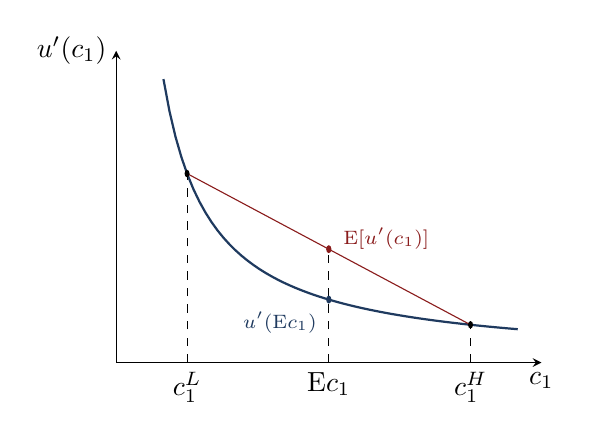
\begin{tikzpicture}[xscale=0.6,yscale=0.9,>=stealth]
  \draw[->] (0,0) -- (9,0) node[below] {$c_1$};
  \draw[->] (0,0) -- (0,4.4) node[left] {$u'(c_1)$};
  \draw[thick,ink,domain=1:8.5,samples=60] plot (\x,{4/\x});
  \draw[key] (1.5,2.667) -- (7.5,0.533);
  \fill (1.5,2.667) circle (1.5pt); \fill (7.5,0.533) circle (1.5pt);
  \draw[dashed] (1.5,0) node[below] {$c_1^L$} -- (1.5,2.667);
  \draw[dashed] (7.5,0) node[below] {$c_1^H$} -- (7.5,0.533);
  \draw[dashed] (4.5,0) node[below] {$\E c_1$} -- (4.5,1.6);
  \fill[key] (4.5,1.6) circle (1.6pt); \fill[ink] (4.5,0.889) circle (1.6pt);
  \node[key,right] at (4.6,1.75) {\scriptsize $\E[u'(c_1)]$};
  \node[ink,below left] at (4.45,0.85) {\scriptsize $u'(\E c_1)$};
\end{tikzpicture}}

% 8. McCall reservation wage
\newcommand{\figMcCall}{%
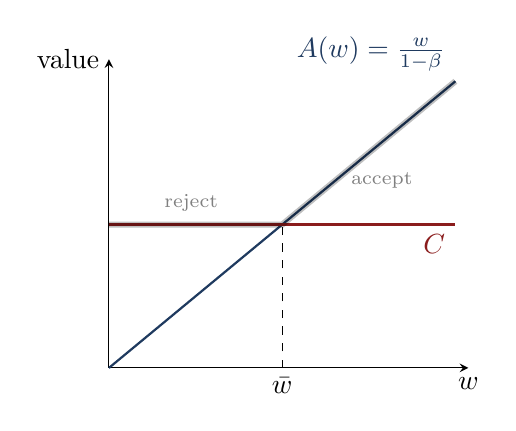
\begin{tikzpicture}[xscale=0.55,yscale=0.7,>=stealth]
  \draw[->] (0,0) -- (8.3,0) node[below] {$w$};
  \draw[->] (0,0) -- (0,5.6) node[left] {value};
  \draw[thick,ink] (0,0) -- (8,5.2) node[above left] {$A(w)=\frac{w}{1-\beta}$};
  \draw[thick,key] (0,2.6) -- (8,2.6) node[below left] {$C$};
  \draw[dashed] (4,0) node[below] {$\bar w$} -- (4,2.6);
  \draw[line width=2.2pt,opacity=0.25] (0,2.6) -- (4,2.6) -- (8,5.2);
  \node[gray] at (1.9,3.0) {\scriptsize reject};
  \node[gray] at (6.3,3.4) {\scriptsize accept};
\end{tikzpicture}}


\newcounter{qn}
\newcommand{\question}[1]{\refstepcounter{qn}\par\medskip
{\bfseries\color{ink}Question \theqn.\ #1}\par\smallskip}

\begin{document}

\begin{center}
{\LARGE\bfseries\color{ink} ECON 5040 Sample Midterm: Short Answers}\\[3pt]
{\small Same ten questions as \texttt{ECON5040\_Sample\_Midterm.pdf}, each answered in two sentences plus the graph to draw (if any).}
\end{center}

\question{Inter-temporal prices}
Explain how the real interest rate determines the relative price of consumption today and consumption in the future. Then explain the substitution incentive created by an increase in the real interest rate.

\begin{answer}
\begin{minipage}[t]{0.58\textwidth}\vspace{0pt}
The gross real interest rate $R=1+r$ is the relative price of consumption today in units of future consumption: giving up one unit of $c_0$ buys $R$ units of $c_1$, so future consumption costs $1/R$ and the budget line $c_0+c_1/R=e_0+e_1/R$ has slope $-R$. A rise in $R$ makes future consumption cheaper (the budget line steepens through the endowment), so the substitution effect always pushes the household to consume less today and save more.
\end{minipage}\hfill
\begin{minipage}[t]{0.38\textwidth}\vspace{0pt}\centering
\scalebox{0.85}{\figIntertemporal}
\end{minipage}
\end{answer}

\question{Choice under uncertainty}
A consumer with $u(c)=\log c$ faces a gamble paying $c=50$ or $c=150$ with equal probability. Compute and interpret the certainty equivalent, and explain how the curvature of $u$ affects the value of this risky prospect.

\begin{answer}
\begin{minipage}[t]{0.58\textwidth}\vspace{0pt}
The certainty equivalent solves $u(CE)=\E u(C)=\tfrac12\log50+\tfrac12\log150$, so $CE=\sqrt{50\cdot150}\approx\mathbf{86.60}$: the consumer would accept 86.60 for sure instead of a gamble with mean 100 (risk premium 13.40). Because $\log$ is concave, losses hurt more than equal gains help ($\E u(C)<u(\E C)$), and the more curved $u$ is, the lower the $CE$ and the larger the risk premium.
\end{minipage}\hfill
\begin{minipage}[t]{0.38\textwidth}\vspace{0pt}\centering
\scalebox{0.85}{\figCE}
\end{minipage}
\end{answer}

\question{Markov processes}
State the Markov property. For a worker whose status follows $P=\begin{bmatrix}0.90&0.10\\0.40&0.60\end{bmatrix}$ (state 1 = employed, state 2 = unemployed), interpret the element $P_{21}$ and the first row of $P$.

\begin{answer}
The Markov property says that, given today's state, the past adds no information about tomorrow's state: $\Pr(X_{t+1}=j\mid X_t=i,X_{t-1},\dots)=\Pr(X_{t+1}=j\mid X_t=i)$. $P_{21}=0.40$ is the probability that an unemployed worker finds a job next period (the job-finding rate), and row 1, $(0.90,0.10)$, is the full distribution of tomorrow's status for an employed worker, so it sums to one.
\end{answer}

\question{Introduction to dynamic programming}
Write the Bellman equation and explain how it decomposes a dynamic problem. For the optimal growth problem ($c_t+k_{t+1}=Ak_t^\alpha$, utility $\sum\beta^t\log c_t$), identify the state variable, choice variable, current payoff, and next-period state.

\begin{answer}
The Bellman equation $V(x)=\max_u\{r(x,u)+\beta\E[V(x')\mid x,u]\}$ splits an infinite-horizon problem into one choice today, valued as the current reward plus the discounted expected value of the state it leads to. In optimal growth the state is $k_t$, the choice is $k_{t+1}$, the current payoff is $\log(Ak_t^\alpha-k_{t+1})$, and the next state is $k'=k_{t+1}$, so $V(k)=\max_{k'}\{\log(Ak^\alpha-k')+\beta V(k')\}$.
\end{answer}

\question{Value functions and policy functions}
Distinguish the value function from the policy function. What economic information does each provide, and how is the optimal policy related to the Bellman equation?

\begin{answer}
The value function $V(x)$ gives how good it is to be in state $x$ when behaving optimally from now on (welfare), while the policy function $h(x)$ gives what to do in each state (behavior, a contingent plan). The optimal policy is the argmax of the Bellman equation, $h(x)=\arg\max_u\{r(x,u)+\beta\E[V(x')\mid x,u]\}$, and $V$ is the value of following $h$ forever.
\end{answer}

\question{Howard's method versus value function iteration}
Explain the logic of value function iteration and of Howard's policy-improvement method. Why can Howard's method be much faster?

\begin{answer}
Value function iteration starts from a value guess and repeatedly applies the Bellman operator $V_{n+1}=TV_n$ until $V$ stops changing, shrinking the error only by a factor of about $\beta$ each step. Howard's method starts from a policy guess, evaluates it exactly with one linear solve $V_h=(I-\beta P_h)^{-1}r_h$, then improves the policy by an argmax and stops when the policy is unchanged, which is fast because each evaluation replaces infinitely many VFI steps and there are only finitely many policies.
\end{answer}

\question{The Solow model}
Explain how saving and capital accumulation determine steady-state capital and output in the Solow model. Does a permanent increase in the saving rate permanently raise the growth rate of output per worker?

\begin{answer}
\begin{minipage}[t]{0.58\textwidth}\vspace{0pt}
Capital grows when investment $sf(k)$ exceeds depreciation $\delta k$, and diminishing returns make the economy converge to the steady state $sf(k^*)=\delta k^*$, i.e.\ $k^*=(sA/\delta)^{1/(1-\alpha)}$ and $y^*=A(k^*)^\alpha$. A higher $s$ raises $k^*$ and $y^*$ (a level effect) with only temporarily faster growth; long-run growth of output per worker is set by technological progress $g$, not by saving.
\end{minipage}\hfill
\begin{minipage}[t]{0.38\textwidth}\vspace{0pt}\centering
\scalebox{0.8}{\figSolow}
\end{minipage}
\end{answer}

\question{Optimal saving}
Interpret the Euler equation $u'(c_t)=\beta R\,\E_t[u'(c_{t+1})]$. How does a household adjust if $u'(c_t)>\beta R\,\E_t[u'(c_{t+1})]$?

\begin{answer}
The left side is the marginal utility of consuming one more unit today, and the right side is the discounted expected marginal utility of saving it instead (it becomes $R$ units tomorrow); at an optimum the two must be equal. If the left side is larger, consuming today is worth more than saving, so the household consumes more and saves less, which lowers $u'(c_t)$ and raises $u'(c_{t+1})$ until they are equal (unless a borrowing constraint binds).
\end{answer}

\question{Income fluctuations}
Explain why uncertainty about future income can increase saving even when expected future income is unchanged, and why assets provide self-insurance.

\begin{answer}
\begin{minipage}[t]{0.58\textwidth}\vspace{0pt}
With convex marginal utility ($u'''>0$), more income risk raises $\E[u'(c_1)]$ above $u'(\E c_1)$, so the Euler equation calls for more saving even though expected income is unchanged: this is precautionary saving. Assets self-insure because the household can draw them down after a bad income draw, shifting resources toward the future states where consumption is low and marginal utility is high.
\end{minipage}\hfill
\begin{minipage}[t]{0.38\textwidth}\vspace{0pt}\centering
\scalebox{0.85}{\figPrecaution}
\end{minipage}
\end{answer}

\question{Putting the ideas together: job search}
Explain why job search is a dynamic decision problem. Formulate the McCall problem in terms of the state variable, choice variable, transition, and continuation value, and explain the reservation wage.

\begin{answer}
\begin{minipage}[t]{0.58\textwidth}\vspace{0pt}
Job search is dynamic because rejecting an offer changes both today's payoff ($c$ instead of $w$) and tomorrow's opportunities (a new draw $W'\sim F$); the state is the offer $w$, the choice is accept or reject, and $V(w)=\max\{w/(1-\beta),\ C\}$ with continuation value $C=c+\beta\E V(W')$. Since the value of accepting rises with $w$ while $C$ is constant, the worker accepts iff $w\ge\bar w=(1-\beta)C$, the reservation wage.
\end{minipage}\hfill
\begin{minipage}[t]{0.38\textwidth}\vspace{0pt}\centering
\scalebox{0.85}{\figMcCall}
\end{minipage}
\end{answer}

\end{document}
